\chapter{RespVis Usage}
\label{chap:Usage}

This chapter discusses how different responsive patterns can be
implemented using the modules provided by the various RespVis packages
outlined in Chapter~\ref{chap:Packages}. The \code{src/examples}
directory of the RespVis library contains examples showing how the
library can be used to create different kinds of charts with varying
degrees of responsiveness. Even though users can compose custom charts
using low-level modules like Series, Axes, and Legends, all the
examples in this chapter focus on creating responsive visualizations
using higher-level Chart Windows. Chart Windows represent convenient
interfaces which allow visualization authors to focus on responsive
configuration, rather than on laborious tasks like setting up a
Chart's structure and handling their render process.

All the example visualizations provided by the RespVis library follow
the same basic structure, outlined in
Listing~\ref{list:ExampleStructure}, namely:
\begin{enumerate}
\item Import the RespVis CSS file \code{respvis.css}. This file
  contains the necessary default styling of visualizations rendered by
  the RespVis library [Line 3].

\item Import D3 and RespVis. RespVis is a D3 extension library, and
  therefore the functionality of both libraries needs to be imported
  from either IIFE or ES modules to create visualizations with
  RespVis [Lines 9 and 11].

\item Attach a new \elname{<div>} element to the root \elname{<div>}
  element (the one with \code{id=\"chart\"}) [Line 14].

\item Bind a fully-initialized data object to the \elname{<div>} element,
  containing the render configuration of the Chart Window. This data
  object is usually created by deriving default properties from a
  partial object via one of the \code{chartWindowXData} functions [Lines 12 and 15].

\item Render the Chart Window using the appropriate
  \code{chartWindowXRender} function [Line 16].

\item Attach a \code{resize} event listener to the \elname{<div>}
  element. This event listener should update the Chart Window's bound
  data object based on media queries and rerender it. Theoretically,
  it is possible to use the actual viewport size in pixels for
  responsive configuration decisions, but it is strongly recommended
  to use media queries via the \code{window.matchMedia} function
  instead. Using media queries allows a Chart's JavaScript
  configuration to be based on the same media queries that might be
  used for the CSS configuration of the same Chart [Line 17].
\end{enumerate}



\begin{samepage}
\lstinputlisting[%
  float=tp,
  aboveskip=\floatsep,
  belowskip=\floatsep,
  xleftmargin=0cm,              % no extra margins for floats
  xrightmargin=0cm,             % no extra margins for floats
  %
  basicstyle=\footnotesize\ttfamily,
  frame=shadowbox,
  numbers=left,
  label=list:ExampleStructure,
  caption={[Structure of Examples]%
The basic structure of all responsive examples provided by RespVis.
Some parts have been removed, so as not to distract the essential parts.
},
]{listings/example-structure.html}
\end{samepage}



Since one of the core premises of RespVis is to enable the
configuration of SVG-based visualizations with CSS, many responsive
patterns can be implemented without JavaScript. In general, everything
which does not affect the content or behavior of a Chart should be
handled in CSS, including the configuration of presentation attributes
and the layout of laid-out elements. Configuration changes which
affect a Chart's content or behavior, like changing the visualized
data, texts, or interaction mechanisms, still need to be applied in
JavaScript. Knowing what kind of configuration is better done in CSS
or JavaScript is not immediately obvious and can be confusing to
figure out for developers unfamiliar with RespVis. There are plans to
allow configuring even more in CSS, but this would require extensive
redesign and refactoring and, therefore, will be considered for a
future release of the library.






\section{Axes}
\label{sec:AxesUsage}

Axes are used to visualize the spatial mapping of abstract values, by
rendering abstract values as ticks at the appropriate spatial
positions to which they are being mapped. In addition to ticks, an
Axis also contains an optional title and an optional subtitle to
describe the axis. Axis-related responsive patterns are of great
importance, since nearly every Chart includes Axes, and often
improving their responsiveness alone can already significantly improve
a visualization consumer's experience.

The following responsive patterns can be applied to Axes in RespVis
visualizations:
\begin{itemize}
\item \liintro{Rotate tick labels}: One of the most effective ways to
  prevent tick labels from overlapping is rotating them by up to 90
  degrees. All the available information is preserved and only
  presented differently. Tick labels can be rotated by setting a
  rotation in the CSS \cssname{transform} property on them and modifying
  their CSS \cssname{text-anchor} property accordingly.

\item \liintro{Simplify tick labels}: In some cases, rotating tick
  labels may not be desired, or labels might still overlap after
  rotation. The next best thing in these cases is to shorten the tick
  labels, if shorter textual representations exist. The D3 Axis
  object used for rendering ticks is accessible via the
  \code{configureAxis} function property on an Axis' data object. How
  exactly tick labels are shortened is specified as a formatting
  callback set via the D3 Axis' \code{tickFormat} function.

\item \liintro{Remove ticks}: If neither rotation nor shortening of
  tick labels is applicable, the last thing that can be done is to
  reduce the number of ticks shown. This can be achieved either via a
  D3 Axis' \code{ticks} or \code{tickValues} function, or via the CSS
  \cssname{display} property. A D3 Axis' \code{ticks} function allows
  specifying the desired number of ticks that shall be rendered, and
  the D3 Axis' render function decides how many ticks to create based
  on this number and other contributing factors. The \code{tickValues}
  function of a D3 Axis allows for much more control than the
  \code{ticks} function, because it is used to specify the exact
  values for which ticks shall be rendered.

\item \liintro{Simplify title/subtitle}: Since Axes do not just
  contain ticks, but also optional titles and subtitles, these should
  not be ignored when optimizing the responsiveness of Axes. Titles
  and subtitles can be simplfied by specifying shorter text strings
  via the \code{title} and \code{subtitle} properties on Axes' data
  objects.

\item \liintro{Relocate title/subtitle}: The titles and subtitles of
  Axes can be relocated by modifying the Axes' grid layouts via the
  CSS \cssname{grid-template} property.

\item \liintro{Remove title/subtitle}: The titles and subtitles of
  Axes can be hidden via the CSS \cssname{display} property.
\end{itemize}





\section{Legends}
\label{sec:LegendsUsage}

Legends visualize the non-spatial mapping of abstract values such as
mappings to colors, shapes, and sizes via labeled symbols. They are
used to explain a visual encoding to a viewer and are frequently
encountered. As such, Legends must not be ignored when optimizing a
visualization's responsiveness.

The following responsive patterns can be applied to Legends in RespVis
visualizations:
\begin{itemize}
\item \liintro{Relocate Legend}: A Legend's position in its containing
  Chart can be controlled by directly modifying the Chart's grid
  layout via the CSS \cssname{grid-template} property, or by positioning
  the Legend at predefined \code{\"top\"}, \code{\"right\"},
  \code{\"bottom\"}, and \code{\"left\"} positions via the
  \attrname{data-legend-position} attribute.

\item \liintro{Simplify title}: A Legend's title can be shortened by
  specifying a shorter text string for it via the \code{title}
  property on a Chart's data object.

\item \liintro{Remove title}: If the title cannot be further
  shortened, or if it does not convey too much important information,
  it can be hidden via the CSS \cssname{display} property.

\item \liintro{Simplify symbol labels}: If the symbol labels can be
  shortened, this can be done via the \code{labels} property on a
  Legend's data object. This property allows the specification of the
  text strings of all labels as an array of string values.

\item \liintro{Relocate labeled symbols}: Changing the layout of
  labeled symbols is one of the most effective responsive patterns
  applicable to Legends. By default, labeled symbols are laid out
  using CSS Flexbox layouting. Thus, whether labeled symbols are laid
  out horizontally or vertically can be controlled using the CSS
  \cssname{flex-direction} property on their container element.
\end{itemize}






\section{Bar Charts}
\label{sec:BarChartsUsage}

Bar charts are used to compare categories associated with quantitative
values by visualizing them as bars whose lengths depend on the
quantitative dimension of the data. In the case of multi-series bar
charts, like grouped bar charts and stacked bar charts, categories are
further divided into subcategories associated with quantitative values
and compared with one another rather than categories themselves. Bars
in a multi-series bar chart are usually colored based on their
subcategories, which is why these charts often include a legend to
explain the color coding.



The different responsive patterns applicable to bar charts have
already been discussed in Section~\ref{sec:BarChartExamples}, and the
focus here lies on demonstrating their implementation using RespVis
Bar Chart Windows. Listing~\ref{list:BarChartPatterns} demonstrates
how some of these patterns can be implemented to create the responsive
Bar Chart shown in Figure~\ref{fig:BarChartPatterns}. In practice, the
responsive patterns which can be applied to different variants of Bar
Charts are very similar, which is why this section does not
differentiate between them.


The following responsive patterns can be applied to RespVis Bar Charts:
\begin{itemize}
\item \liintro{Rescale draw area}: Scaling a Bar Chart to fit into the
  available space is done automatically by their render functions. By
  default, Axes and Legends only take up as much space as necessary,
  and the remaining space is filled with the Chart's draw area. Bars
  and labels in this draw area are automatically scaled and positioned
  to fit into the allocated space.

\item \liintro{Reduce bar padding}: Reducing the padding between bars
  frees up space that can be used by the bars themselves. Padding
  can be controlled via the \code{padding} function on the
  \code{categoryScale} property of a Bar Chart's data object.

\item \liintro{Simplify bar labels}: When reducing the width of Bar
  Charts, bar labels might start overlapping one another, and it might
  be a good idea to shorten them, if possible. Bar labels can be
  configured using the \code{labels} property of a Bar Chart's data
  object.

\item \liintro{Remove bar labels}: An alternative to prevent bar
  labels from overlapping is to hide some or even all of them. The
  best way of implementing this is to hide them via the CSS
  \cssname{opacity} or \cssname{display} properties.

\item \liintro{Transpose Chart}: By default, a Bar Chart is rendered
  with vertical bars, transposing it would make the bars horizontal.
  Horizontal Bar Charts are better suited for narrow spaces, because
  the bar labels and Axis tick labels of the categories are easier to
  place. Furthermore, Horizontal Bar Charts are allowed to extend
  outside the visible viewport because vertical scrolling is more
  acceptable than horizontal scrolling. A Bar Chart can be transposed
  by setting the \code{flipped} property on its data object.

\item \liintro{Remove bars}: Sometimes it might be required to reduce
  the number of bars to maintain a good visualization consumer
  experience. Bars representing certain categories or subcategories
  can be hidden by declaring them as inactive via the
  \code{activeCategories} and \code{activeSubcategories} properties on
  a Bar Chart's data object. Using these properties is easier than
  manually adapting the \code{categories}, \code{values},
  \code{categoryScale}, and \code{valueScale} properties on the data
  object. Furthermore, categories and subcategories which have been
  hidden via the \code{activeCategories} and
  \code{activeSubcategories} properties can also be unhidden by
  consumers via a Chart's Toolbar, if they wish to see the additional
  data.

\item \liintro{Apply Axis patterns}: Since a Bar Chart usually
  contains two Axes to visualize the spatial mappings of categories
  and values, all the responsive patterns described in
  Section~\ref{sec:AxesUsage} can and should be applied to Bar Charts.

\item \liintro{Apply Legend patterns}: For a Multi-Series Bar Chart
  containing a Legend, the responsive patterns mentioned in
  Section~\ref{sec:LegendsUsage} can and should be applied.
\end{itemize}



\begin{samepage}
\lstinputlisting[%
  float=tp,
  aboveskip=\floatsep,
  belowskip=\floatsep,
  xleftmargin=0cm,              % no extra margins for floats
  xrightmargin=0cm,             % no extra margins for floats
  %
  basicstyle=\footnotesize\ttfamily,
  frame=shadowbox,
  numbers=left,
  label=list:BarChartPatterns,
  caption={[Implementation of a Responsive RespVis Bar Chart]%
The implementation of the responsive Bar Chart shown in
Figure~\ref{fig:BarChartPatterns}. Depending on the available width,
Axis tick labels are rotated, bar labels are simplified, and on very
narrow screens, the whole Chart is transposed. Non-essential parts
have been removed for clarity.
},
]{listings/bar-chart-patterns.html}
\end{samepage}





\begin{figure}[tp]
\newcommand{\respscale}{0.54}
%\centering
\subfloat[][60rem]{%
  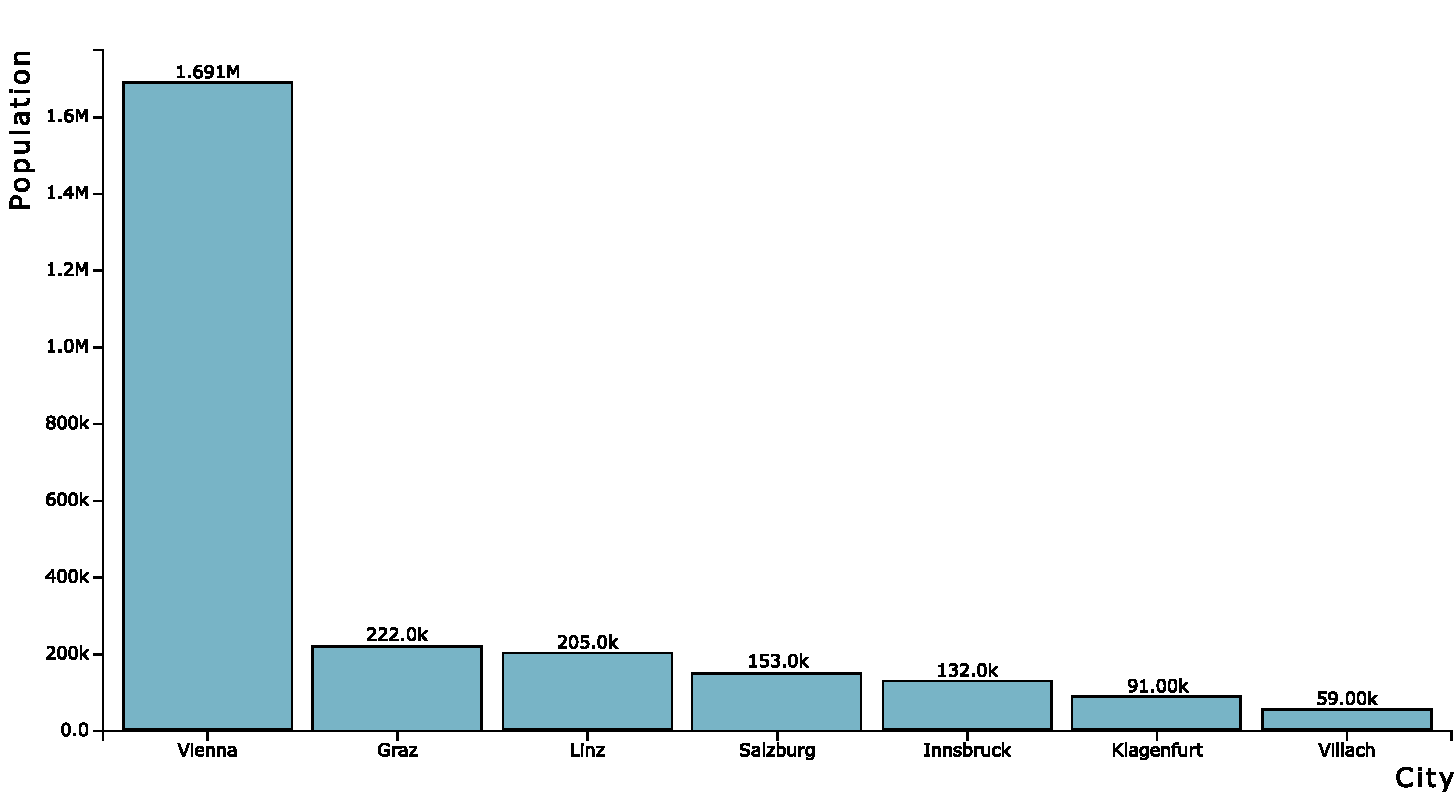
\includegraphics[valign=b,scale=\respscale]{diagrams/respvis-bar-60rem.pdf}%
  \label{fig:BarChartPatterns60rem}%
}
\\[2mm]
\subfloat[][40rem]{%
  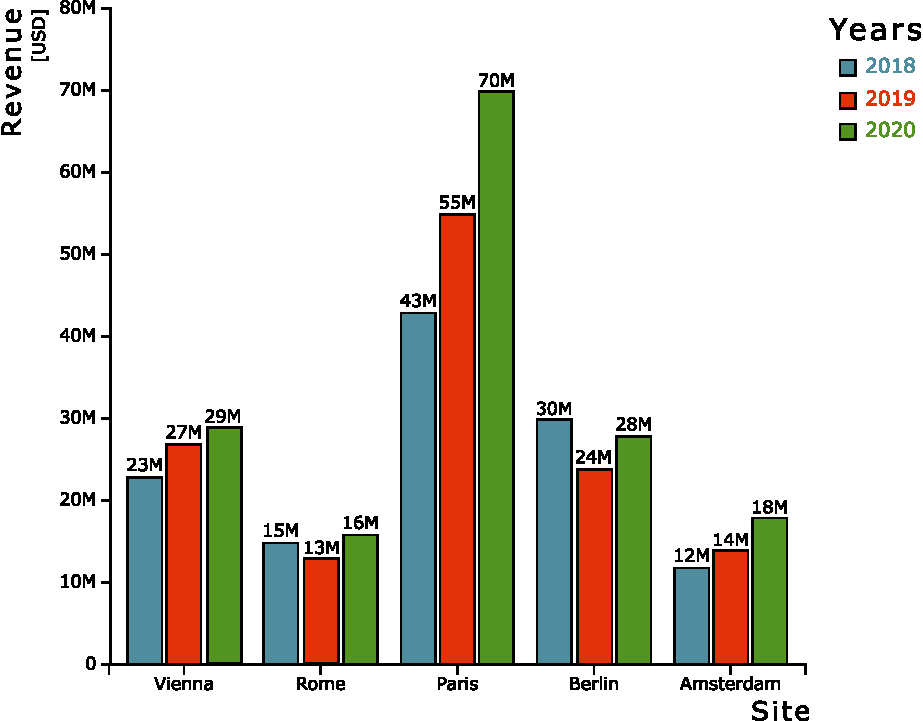
\includegraphics[valign=b,scale=\respscale]{diagrams/respvis-bar-40rem.pdf}%
  \label{fig:BarChartPatterns40rem}%
}
\hfill
\subfloat[][30rem]{%
  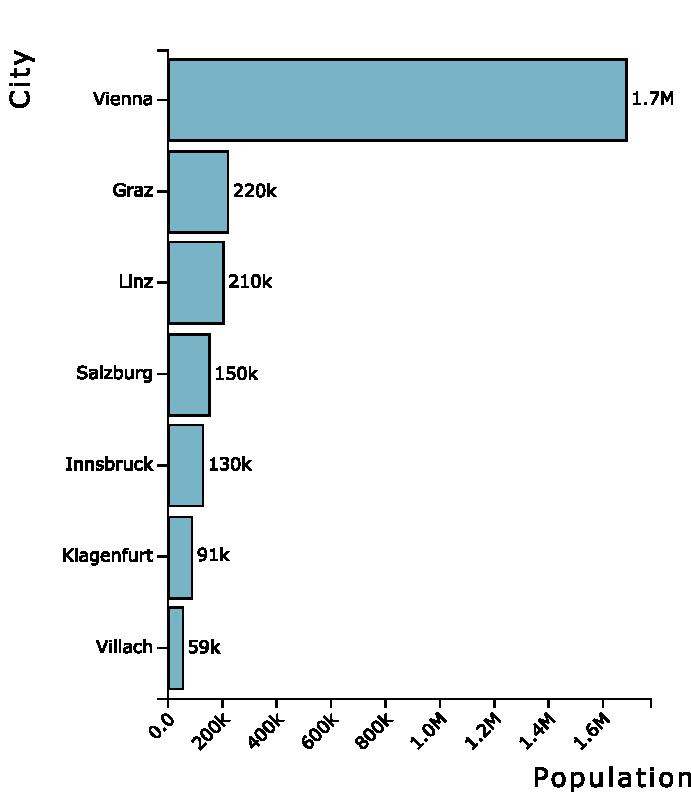
\includegraphics[valign=b,scale=\respscale]{diagrams/respvis-bar-30rem.pdf}%
  \label{fig:BarChartPatterns30rem}%
}
\caption[Responsive RespVis Bar Chart]{%
The responsive Bar Chart resulting from the implementation in
Listing~\ref{list:BarChartPatterns}.
\subref{fig:BarChartPatterns60rem} At a width of 60rem, the
Chart is not yet transposed, bar labels are shown above the bars with
four digits of precision, and the bottom axis tick labels are not
rotated. \subref{fig:BarChartPatterns40rem} At a width of
40rem, bar labels are shown with three digits of precision, and the
bottom axis tick labels are rotated by 45 degrees.
\subref{fig:BarChartPatterns30rem} At a width of 30rem, the
Chart is transposed, bar labels are shown with two digits of precision
to the right of bars, and the (newly) bottom axis tick labels are
rotated by 45 degrees.
\imgcredit{Image created by the author of this thesis using RespVis.}
}
\label{fig:BarChartPatterns}
\end{figure}









\section{Line Charts}
\label{sec:LineChartsUsage}

Line charts are visualizations which show trends in data by plotting
markers at regular intervals and connecting them with lines.
Single-series line charts show trends in two-dimensional data via a
single line and multi-series line charts show trends in
multi-dimensional data via multiple lines. The different lines in a
multi-series line chart can be seen as representations of
subcategories in the data and are usually colored differently to
reflect this. For this reason, a multi-series line chart typically
includes a legend to explain the color coding of subcategories.


The responsive patterns applicable to line charts have already been
discussed in Section~\ref{sec:LineChartExamples}. The focus here lies
in demonstrating how they can be implemented using RespVis Line Chart
Windows. Listing~\ref{list:LineChartPatterns} demonstrates how some of
these patterns can be combined to create the responsive Line Chart
shown in Figure~\ref{fig:LineChartPatterns}.


The following responsive patterns can be applied to RespVis Line Charts:
\begin{itemize}
\item \liintro{Rescale draw area}: As for Bar Charts, Line Charts are
  automatically scaled by their render functions. The default behavior
  is that Axes and potential Legends only take up as much space as
  necessary, and whatever space is left is filled with the Chart's
  draw area. Elements contained in the draw area like lines,
  markers, and labels are automatically scaled and positioned to fit
  into the available space.

\item \liintro{Remove markers}: If a Chart contains a large number of
  individual data points, visual clutter can be reduced by not showing
  markers for every single data point. The best way to remove markers
  is to hide them via the CSS \cssname{opacity} or \cssname{display}
  properties.

\item \liintro{Rescale markers}: An alternative to removing markers is
  to decrease their size. Marker sizes can be controlled via the
  \code{markers.radiuses} property on the data objects of Line Charts.

\item \liintro{Simplify marker labels}: The labels of markers might
  start overlapping when trying to fit a Line Chart into increasingly
  narrow widths. A good solution for this is to shorten marker labels
  by providing shorter text strings for them via the \code{labels}
  property on the Line Chart's data object.

\item \liintro{Remove marker labels}: Sometimes, shortening marker
  labels may not be possible, desired, or effective enough. An
  alternative to prevent them from overlapping is to remove some or
  all of them. The recommended way to remove marker labels is to hide
  them via the CSS \cssname{opacity} or \cssname{display} properties.

\item \liintro{Transpose Chart}: Even though Line Charts are less
  frequently transposed than Bar Charts, there are still situations
  when transposing a Line Chart could improve the visualization
  consumer's experience. One such situation would be a Line Chart with
  so many data points that a Horizontal Line Chart with limited width
  is too dense. Transposing such a chart into a Vertical Line Chart
  might reduce the data density by allowing the Chart to extend
  outside the visible viewport and having consumers scroll vertically.
  Furthermore, Vertical Line Charts are useful for heavily annotated
  Line Charts because labels are much easier to place than in
  horizontal ones. Line Charts can be transposed by setting the
  \code{flipped} property on their data objects.

\item \liintro{Apply Axis patterns}: As with all Charts which use Axes
  to visualize spatial mappings, the responsive patterns described in
  Section~\ref{sec:AxesUsage} can and should be applied to the Axes in
  a Line Chart. The Axes of a Line Chart could even be removed
  completely via the CSS \cssname{display} property, turning the Line
  Chart into a Sparkline, but this should be considered carefully
  because information about the scale is lost when hiding Axes.

\item \liintro{Apply Legend patterns}: Where a Multi-Series Line Chart
  contains a Legend to explain a non-spatial data encoding, the
  responsive patterns discussed in Section~\ref{sec:LegendsUsage} can
  and should be applied.
\end{itemize}




\begin{samepage}
\lstinputlisting[%
  float=tp,
  aboveskip=\floatsep,
  belowskip=\floatsep,
  xleftmargin=0cm,              % no extra margins for floats
  xrightmargin=0cm,             % no extra margins for floats
  %
  basicstyle=\footnotesize\ttfamily,
  frame=shadowbox,
  numbers=left,
  label=list:LineChartPatterns,
  caption={[Implementation of a Responsive RespVis Line Chart]%
The implementation of the responsive Line Chart shown in
Figure~\ref{fig:LineChartPatterns}. Depending on the available width,
Axis ticks and markers are hidden, Axis tick labels are simplified,
and on very narrow screens, Axes are hidden turning the Line Chart
into a Sparkline. Non-essential parts of the implementation have been
removed for clarity.
},
]{listings/line-chart-patterns.html}
\end{samepage}



\begin{figure}[tp]
\newcommand{\respscale}{0.54}
%\centering
\subfloat[][60rem]{%
  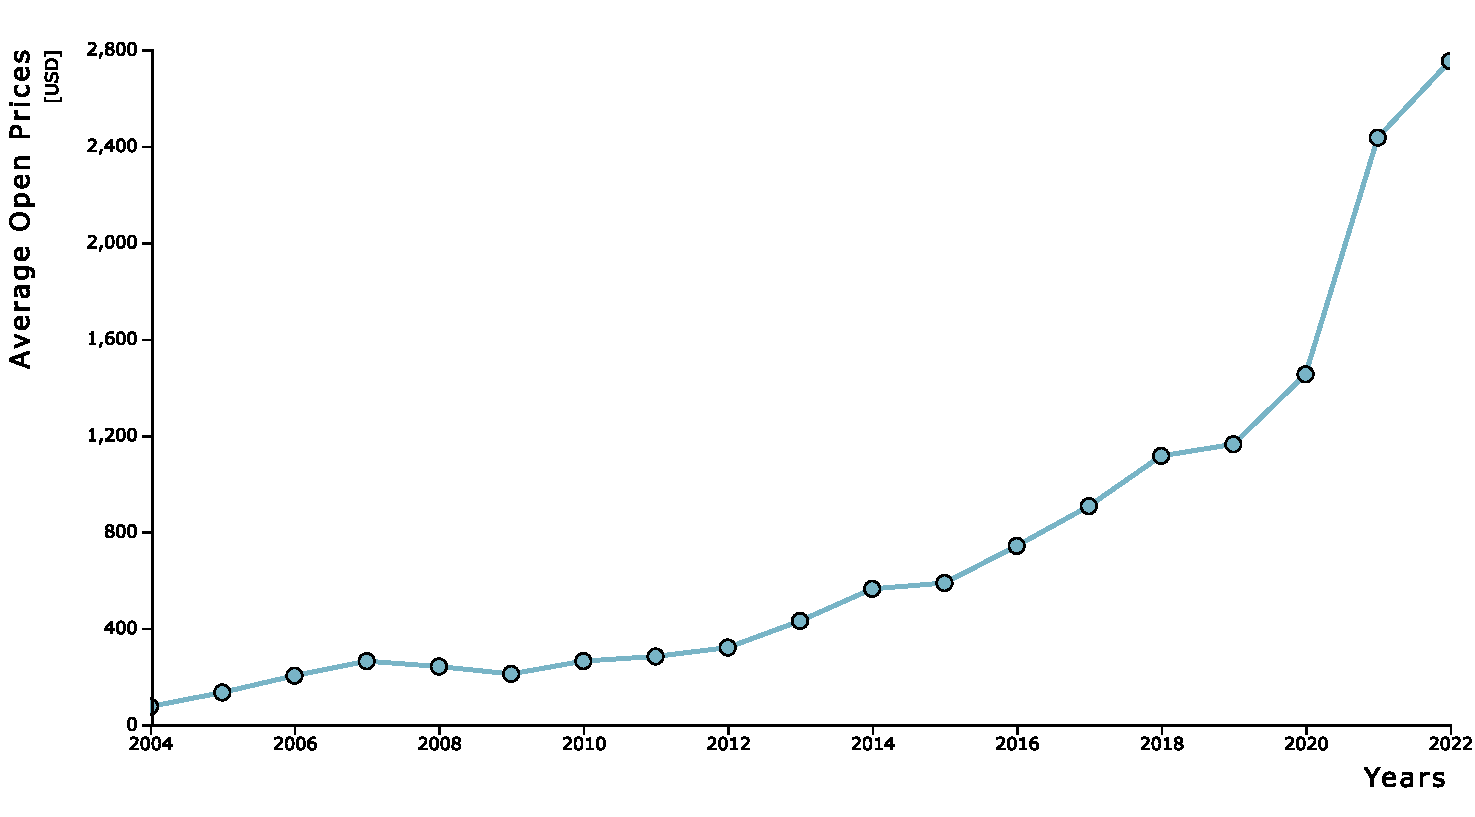
\includegraphics[valign=b,scale=\respscale]{diagrams/respvis-line-60rem.pdf}%
  \label{fig:LineChartPatterns60rem}%
}
\\[2mm]
\subfloat[][40rem]{%
  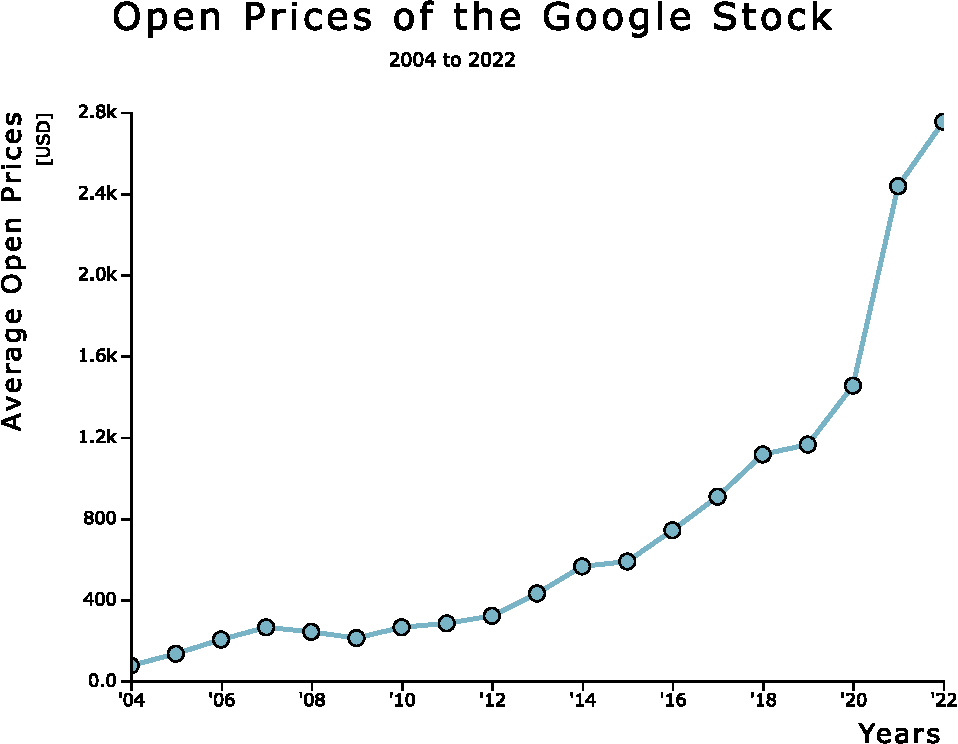
\includegraphics[valign=b,scale=\respscale]{diagrams/respvis-line-40rem.pdf}%
  \label{fig:LineChartPatterns40rem}%
}
\hfill
\subfloat[][30rem]{%
  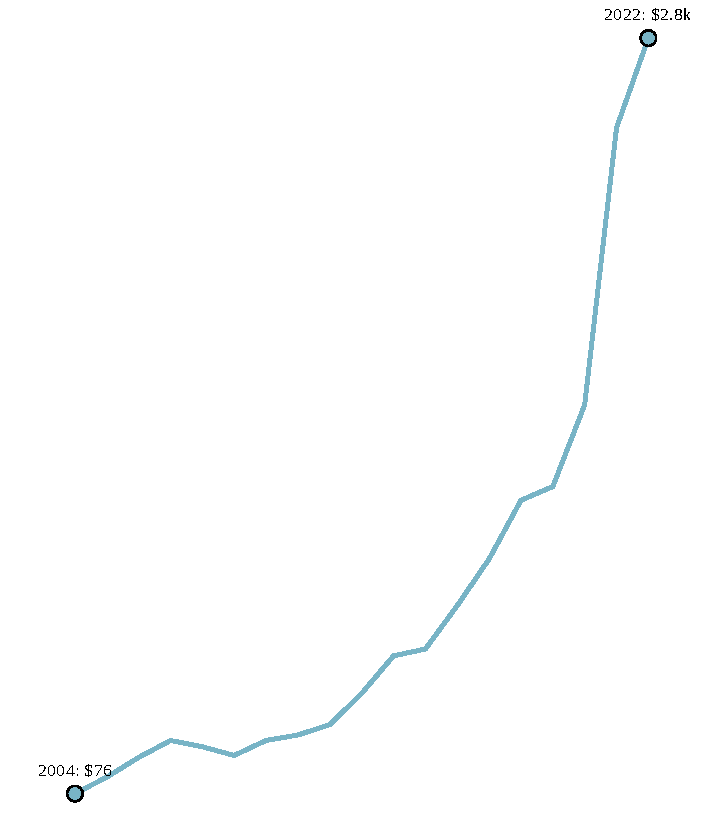
\includegraphics[valign=b,scale=\respscale]{diagrams/respvis-line-30rem.pdf}%
  \label{fig:LineChartPatterns30rem}%
}
\caption[Responsive RespVis Line Chart]{%
The responsive Line Chart resulting from the implementation in
Listing~\ref{list:LineChartPatterns}.
\subref{fig:LineChartPatterns60rem} At a width of 60rem, all markers
are shown and tick labels are not shortened.
\subref{fig:LineChartPatterns40rem} At a width of 40rem, tick labels
are shortened. \subref{fig:LineChartPatterns30rem} At a width of
30rem, axes are hidden, the title is simplified, the subtitle is
hidden, and only the first and last markers and marker labels are
shown, turning the chart into a sparkline.
\imgcredit{Image created by the author of this thesis using RespVis.}
}
\label{fig:LineChartPatterns}
\end{figure}









\section{Point Charts}
\label{sec:PointChartsUsage}

Point charts, sometimes also called scatterplots, are used to discover
patterns and correlations in data by plotting individual data points
as points in a Cartesian coordinate system. Often, point charts are
only used to visualize two-dimensional data by plotting points of the
same color and size, but they can also be used to visualize
multi-dimensional data by adding color, size, or shape encodings. If
such an additional encoding is used, a point chart usually includes a
legend to explain it.

The responsive patterns applicable to point charts have already been
discussed in Section~\ref{sec:ScatterplotExamples}. The focus here
lies on demonstrating their implementation using RespVis Point Chart
Windows. Listing~\ref{list:PointChartPatterns} shows how some of
these patterns can be implemented to create the responsive Point Chart
displayed in Figure~\ref{fig:PointChartPatterns}.


The following responsive patterns can be applied to RespVis Point
Charts:
\begin{itemize}
\item \liintro{Rescale draw area}: As with other Cartesian Charts, the
  draw area of a Point Chart and its contents are automatically
  scaled by the Chart's render functions to fill the space not
  occupied by the Axes and any potential Legend.

\item \liintro{Rescale points}: When a large number of data points are
  rendered in a Point Chart, it can be helpful to reduce their sizes
  to make individual points easier to see and reduce clutter. The
  sizes of points can be controlled via the \code{radiuses} property
  on the data objects of Point Charts.

\item \liintro{Simplify labels}: When labels are shown in a Point
  Chart, it might be helpful to shorten them when reducing the width
  of Charts to prevent them from overlapping. The texts of labels can
  be configured via the \code{labels} property on the data object of
  the Point Chart.

\item \liintro{Remove labels}: Often, Point Charts are used to
  visualize large data sets. In such situations, rendering labels
  for all points would only clutter the visualization, and it might be
  better to hide them via the CSS \cssname{opacity} or \cssname{display}
  properties.

\item \liintro{Zoom draw area}: Zooming allows visualization consumers
  to view data at various levels of detail. A Point Chart can be
  zoomed by adjusting the domains of the scales handling the spatial
  encoding of data, which are the \code{xScale} and \code{yScale}
  properties of the data object of the Point Chart. To simplify the
  setup and handling of zooming interaction, the D3 Zoom package
  \parencite{D3Zoom} can be used, which is illustrated in
  Listing~\ref{list:PointChartPatterns}.

\item \liintro{Apply Axis patterns}: As with all Charts which use Axes
  to visualize spatially-encoded data, the responsive patterns
  described in Section~\ref{sec:AxesUsage} can and should be applied
  to Point Charts.

\item \liintro{Apply Legend patterns}: Where a Point Chart visualizes
  an additional non-spatial data encoding with a Legend, the
  responsive patterns discussed in Section~\ref{sec:LegendsUsage} can
  and should be applied.
\end{itemize}







\begin{samepage}
\lstinputlisting[%
  float=tp,
  aboveskip=\floatsep,
  belowskip=\floatsep,
  xleftmargin=0cm,              % no extra margins for floats
  xrightmargin=0cm,             % no extra margins for floats
  %
  basicstyle=\footnotesize\ttfamily,
  frame=shadowbox,
  numbers=left,
  label=list:PointChartPatterns,
  caption={[Implementation of Responsive RespVis Point Charts]%
The implementation of the responsive Point Chart shown in
Figure~\ref{fig:PointChartPatterns}. Depending on the available width,
Axis ticks are hidden, Axis tick labels are shortened, and point
radiuses are reduces. Additionally, zooming is implemented using the
D3 Zoom package \parencite{D3Zoom}. Non-essential parts of the
implementation have been removed for clarity.
},
]{listings/point-chart-patterns.html}
\end{samepage}



\begin{figure}[tp]
\newcommand{\respscale}{0.54}
%\centering
\subfloat[][60rem]{%
  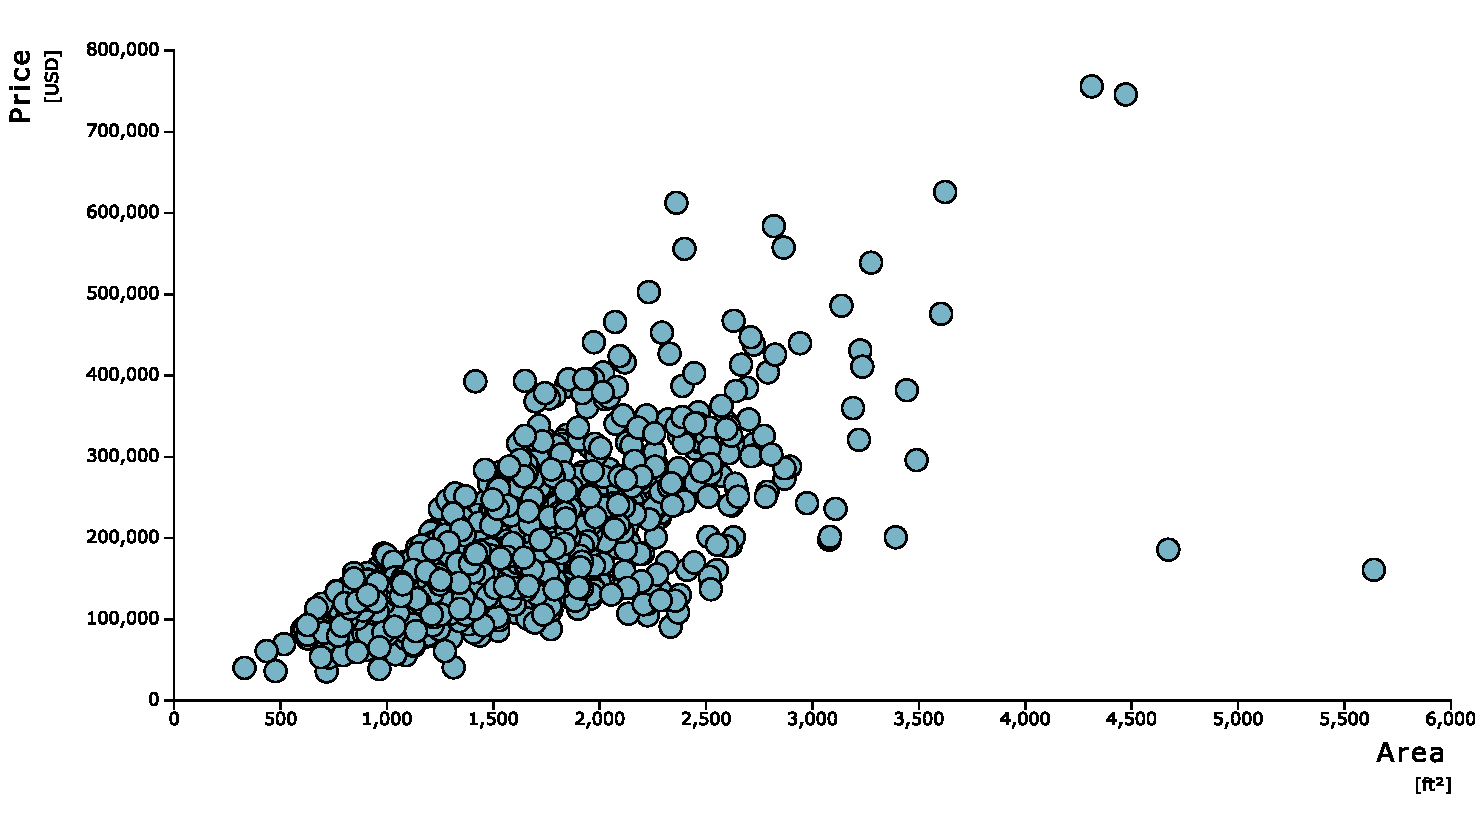
\includegraphics[valign=b,scale=\respscale]{diagrams/respvis-point-60rem.pdf}%
  \label{fig:PointChartPatterns60rem}%
}
\\[2mm]
\subfloat[][40rem]{%
  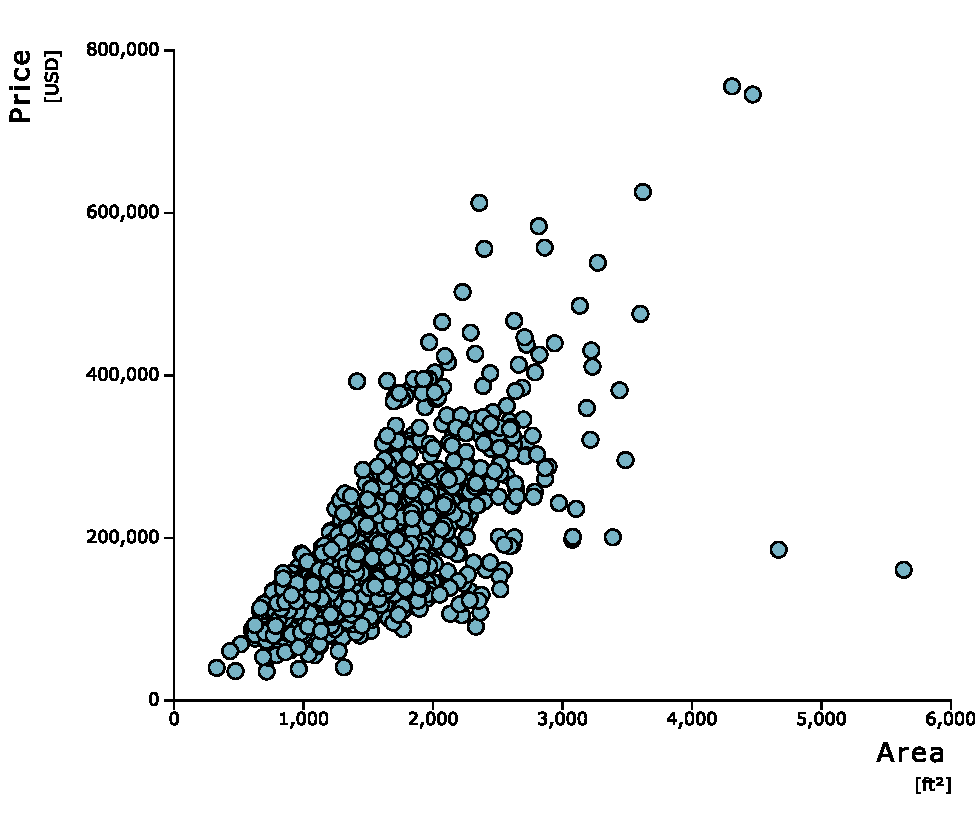
\includegraphics[valign=b,scale=\respscale]{diagrams/respvis-point-40rem.pdf}%
  \label{fig:PointChartPatterns40rem}%
}
\subfloat[][30rem, zoomed]{%
  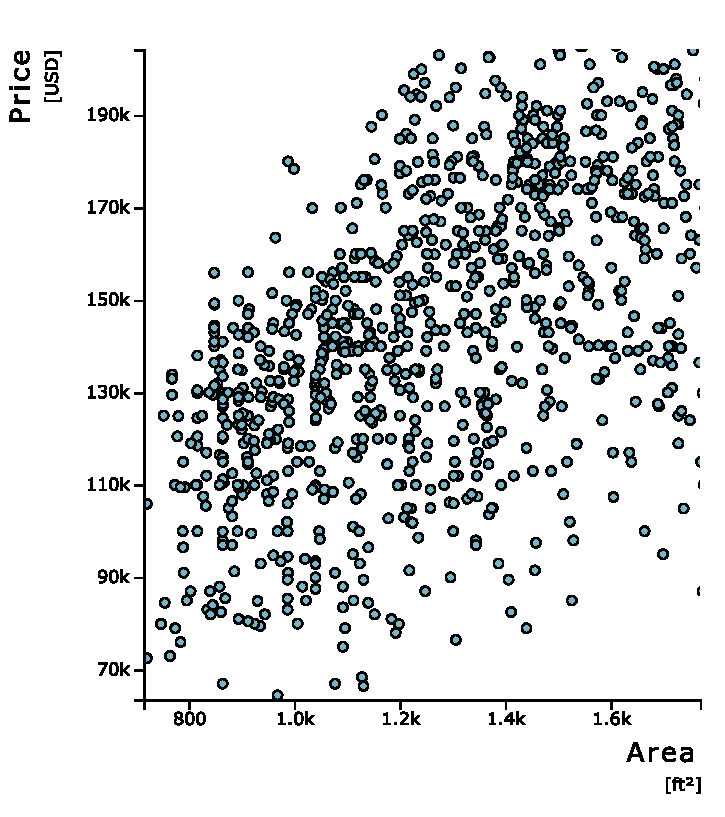
\includegraphics[valign=b,scale=\respscale]{diagrams/respvis-point-30rem-zoomed.pdf}%
  \label{fig:PointChartPatterns30remZoomed}%
}
\caption[Responsive RespVis Point Chart]{%
The resulting responsive Point Chart that is rendered from the
implementation in Listing~\ref{list:PointChartPatterns}.
\subref{fig:PointChartPatterns60rem} At a width of 60rem, all ticks
are shown, tick labels are not shortened, and points are rendered at
their full size. \subref{fig:PointChartPatterns40rem} At a width of
40rem, only every second tick is shown and point sizes are reduced.
\subref{fig:PointChartPatterns30remZoomed} At a width of 30rem, tick
labels are shortened using scientific notation and point sizes are
reduced further. Additionally, the chart has been zoomed in.
\imgcredit{Image created by the author of this thesis using RespVis.}
}
\label{fig:PointChartPatterns}
\end{figure}


